We measure the MCP server ecosystem by \emph{executing} it. This section defines
the sampling frame, the conformance harness, the sandbox, and the grading rules
(Figure~\ref{fig:pipeline}). The harness and the released dataset make every number
reproducible.

\begin{figure*}[t]
  \centering
  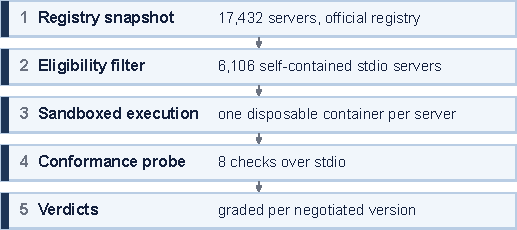
\includegraphics[width=0.85\textwidth]{figures/pipeline.pdf}
  \caption{Measurement pipeline. Every eligible server is installed and executed in
  its own disposable container, then driven through the conformance probe and graded
  against the protocol version it negotiates.}
  \label{fig:pipeline}
\end{figure*}

\subsection{Sampling frame}
We crawl the official MCP registry (\texttt{registry.modelcontextprotocol.io})
via its cursor-paginated API, retaining the latest published version of each
server. This yields \Nframe{} unique servers. Each server declares zero or more
\emph{packages} (installable artifacts on npm, PyPI, OCI, NuGet, or Cargo) and/or
\emph{remotes} (hosted HTTP endpoints). Our study population is the set of servers
that are (i) locally installable, (ii) use the \texttt{stdio} transport, (iii)
distributed on npm or PyPI (the two dominant registries), and (iv)
\emph{self-contained}: they declare no required environment variable or argument
that lacks a default. Criterion (iv) restricts us to servers that a client could
launch without provisioning secrets, which both bounds the ethics of mass
execution and defines a clean, reproducible population. We report the exclusion of
remote-only and credential-requiring servers explicitly (Section~\ref{sec:threats})
and treat the resulting frame as the denominator for all rates. We probe the
\emph{entire} frame (all \Nprobed{} eligible servers), so the measurement is a census of the eligible population.

\subsection{Conformance harness}
The harness, \texttt{mcpprobe}, is a deliberately minimal, hand-written JSON-RPC
client speaking line-delimited messages over the server's stdio. We do \emph{not}
use an official SDK client. To observe raw behavior, including responses to
malformed frames, the probe must not inherit any SDK-side correction or
validation. The harness offers protocol version \texttt{2025-06-18} at
initialization (the then-current revision was \texttt{2025-11-25}), records the
version the server \emph{negotiates}, and grades all later checks against that version. A server that supports the
offered version must answer with it, and \(3{,}576\) of \Nresponders{} responders did,
so almost all grading is against \texttt{2025-06-18}. Responding servers negotiated four distinct
revisions, and \(109\) of them settled on something other than the version we
offered, the oldest dating to 2024-11-05.

Each server is driven through the following checks, whose identifiers align with
the categories of the official \texttt{modelcontextprotocol/conformance} suite
where an analogue exists:

\begin{itemize}
  \item \textbf{server-initialize}: the \texttt{initialize} request must return a
    result carrying a protocol version and a capabilities object; the harness then
    sends \texttt{notifications/initialized}.
  \item \textbf{ping}: a \texttt{ping} must return an empty-object result.
  \item \textbf{tools-list}: if the server advertises the tools capability,
    \texttt{tools/list} must return an array in which every entry has a
    \texttt{name} and an \texttt{inputSchema} object.
  \item \textbf{tools-schema-valid}: each declared \texttt{inputSchema} must be a
    valid JSON Schema (checked by meta-validation).
  \item \textbf{tools-call-unknown}: calling a non-existent tool must be rejected.
    The specification's Error Handling section categorizes ``Unknown tools'' under
    \emph{Protocol Errors} (standard JSON-RPC errors) and illustrates this with a
    \texttt{-32602} example, as opposed to \emph{Tool Execution Errors} reported as
    a result with \texttt{isError: true}. This categorization is prose plus an
    example; it uses no RFC-2119 \textsf{MUST}/\textsf{SHOULD} keyword. We
    therefore do not treat a non-conforming response as a ``violation''; instead we
    record which of the two mechanisms the server uses (see
    \textsf{error-as-result} below).
  \item \textbf{tools-call-invalid-args}: for a tool with a typed required
    property, calling it with a wrong-typed value should be rejected. The spec is
    itself ambiguous here, since it lists ``Invalid arguments'' under Protocol Errors
    but ``Invalid input data'' under Tool Execution Errors, so we count \emph{either} a
    protocol error \emph{or} an \texttt{isError} result as acceptable, and flag only
    a plain success response (the tool ran on ill-typed input) as a defect.
  \item \textbf{malformed-json}: after receiving a syntactically invalid frame, the
    server must not crash or hang; a subsequent \texttt{ping} must still succeed.
  \item \textbf{stdout-purity}: under the stdio transport, the server must emit only
    protocol messages on stdout; any non-JSON line is a channel-corruption defect.
\end{itemize}

\subsection{Grading and the error-as-result category}
Verdicts are \textsf{pass}, \textsf{fail}, \textsf{warn}, \textsf{skip}, and one
category introduced by calibration: \textsf{error-as-result}. When validating the
harness against the official reference servers (\texttt{server-memory},
\texttt{server-everything}), we found they answer an unknown-tool call not with the
specified JSON-RPC \texttt{-32602} error but with a \emph{successful} response whose
\texttt{result.isError} flag is set. Because this behavior originates in the
official SDKs and is therefore ecosystem-wide, we grade it as its own category, not as a failure, and report its prevalence as a result.

\subsection{Sandbox}
Executing thousands of untrusted packages demands isolation. Each server runs in a
fresh container (\texttt{node:22-slim} for npm, an \texttt{astral-sh/uv} image for
PyPI) with a memory cap, a single CPU, a PID limit, \texttt{no-new-privileges}, all
Linux capabilities dropped, and no host filesystem mounts. The harness supports two
probe conditions. In the \textbf{two-phase}
condition, an online install pass populates the cache and the conformance probe then
runs with \texttt{-{}-network=none}, so no server code has network access while it is
being measured. In the \textbf{single-phase} condition, install and probe occur
together in one ephemeral container and the network is available throughout. The
census reported here was measured in the single-phase condition, for the operational
reasons given in Section~\ref{sec:method-env}, and we state the consequences for
validity in Section~\ref{sec:threats}.

\subsection{Execution environment and probe condition}
\label{sec:method-env}
The census was executed on a single disposable cloud instance (no cloud
credentials attached, so the blast radius of running untrusted code is one
throwaway host) using the online single-phase condition: install and probe occur
in one ephemeral \texttt{-{}-rm} container per server, with nothing cached between
servers so that disk usage stays bounded across the full ecosystem; the recorded
launch command of every run confirms that no volume was mounted. We did not run a
controlled comparison of the two conditions. In development runs on smaller subsets,
error-as-result prevalence (\(87\%\)) and silent type non-enforcement (\(7\%\)) among
responding servers were the same under both conditions; handshake yields from those
runs are not comparable, because the subsets differed. Two groups of runs ended for
reasons outside the server's control or of uncertain cause: \(32\) probes
(\(0.5\%\)) were killed (exit 137) by either the memory cap or an automated guard
that reclaims host disk space, and the census does not record which; \(17\) probes
(\(0.3\%\)) aborted on a harness-side error before any check ran. All but one of
these \(49\) are counted as non-handshaking, so they can only lower the handshake
yield; the exception was killed after completing its handshake.

\subsection{SDK-level confirmation}
\label{sec:sdk-probe}
Where a conformance failure concentrates in one SDK family, the census alone cannot
say whether the library permits the failure or the authors introduced it
independently. For the input-validation result we tested the SDK directly. We build two minimal servers exposing one tool that declares a
single required string property, one using the low-level \texttt{Server} API and one
using the high-level \texttt{McpServer} API, both on the same SDK release, and drive
each with the same harness check used in the census: a \texttt{tools/call} carrying an
integer where the declared schema requires a string. The construction is otherwise
identical, so any difference in outcome is a property of the API path. We report the
result in Section~\ref{sec:consequences}. The two servers and the probe script are
released with the harness.

\subsection{Funnel accounting}
Because ``does it even run'' is itself a research question, we count every stage:
declared $\rightarrow$ eligible (self-contained stdio npm/PyPI) $\rightarrow$
container started $\rightarrow$ process launched
$\rightarrow$ handshake completed $\rightarrow$ probed. Servers that never reach a
handshake are classified into startup-failure categories
(Section~\ref{sec:results}) from their exit code and stderr, so that the lost yield can be explained.
